\subsection{问题四的模型的建立和求解}

\subsubsection{具体分析}

针对问题四，本问属于\textbf{技术演进建模与前沿预测}类问题，需要结合历史评测数据建立技术演进模型，分离并量化规模扩张与非规模技术进步的贡献占比，并预测未来 12 至 24 个月开源大语言模型能力的前沿边界\cite{wei2022emergent}。本问综合采用“口径界定 $\to$ Loss—Benchmark 桥接 $\to$ 面板回归分解 $\to$ 前沿预测 $\to$ 宏观证据校验”五步框架：首先明确综合能力的度量方式、开源筛选口径、模型类型口径与时间轴口径；再按可比性分层建立交叉熵损失与 Leaderboard 得分的映射，把前三问以损失为目标的结论桥接到以评测得分为度量的能力；然后以参数规模与年份为解释变量做面板回归（含年份固定效应），把能力提升分解为“规模扩张”与“非规模技术进步”两部分；接着用 logistic 饱和模型与结构外推两条路线给出未来 12/24 个月的前沿预测与不确定性区间；最后用附件 C4 的算力、数据量与开源权重证据检验“算力增长放缓”情景的合理性。

本问严格完成题设的必用要求：对 C8 的逐任务评测 JSON 做逐任务聚合分析（不依赖汇总表），对 C4 的算力、数据量与开源权重字段作宏观证据检验，桥接数据按可比性等级（C6 的 High/Medium，并以 C5 对照）分层使用。

\subsubsection{模型准备}

\textbf{1.口径界定}

\textbf{（1）综合能力度量。} 采用 Open LLM Leaderboard v2 的六维平均分 $\bar B$：IFEval（指令遵循）、BBH（多跳推理）、MATH Lvl 5（数学）、GPQA（研究生级问答）、MUSR（多轮推理）、MMLU-PRO（专业知识）。六维等权平均，取值 $0\sim100$。

\textbf{（2）时间轴口径。} 统一以 C1 的 Submission Date（提交日期）为基准，并按“年 $+$ 月”折算为连续时间变量 $t=\text{年份}-2019+(\text{月}-0.5)/12$。之所以不采用发布日期或版本日期，是因为 Leaderboard 上的评测结果均在提交时冻结、且提交日期字段完整无缺失；C3 的 Year 字段仅用于 2019--2023 的历史锚点对照。

\textbf{（3）开源筛选口径。} 同时要求两个条件：（a）模型权重可获取（Type 属 pretrained、持续预训练、chat、域内微调四类）；（b）Hub License 允许研究与复现，即采用 apache-2.0、mit、gpl-3.0、cc-by-4.0、mpl-2.0、bsd-3-clause、llama2/3/3.1/3.2/3.3、gemma、cc-by-sa-4.0、openrail 等许可，排除 cc-by-nc 系列（非商用）、creativeml-openrail、bigscience-bloom-rail 等受限许可以及未知许可。筛选漏斗见表\ref{tab:p4_funnel}。

\textbf{（4）模型类型口径。} 明确区分 pretrained（含持续预训练，共 231 条）与 chat/finetuned（经对话指令或监督微调，共 1{,}497 条）两类，分组统计规模效应与时间效应；base 合并模型（1{,}724 条，非独立训练过程）与多模态模型（9 条，任务构成不同）不并入主分析。

\begin{longtable}{>{\raggedright\arraybackslash}p{0.56\textwidth}>{\centering\arraybackslash}p{0.16\textwidth}>{\raggedright\arraybackslash}p{0.22\textwidth}}
  \caption{数据筛选漏斗（C1 排行榜）}
  \label{tab:p4_funnel} \\
  \toprule
  筛选层级 & 记录数 & 说明 \\
  \midrule
  \endfirsthead
  \caption{数据筛选漏斗（续）} \\
  \toprule
  筛选层级 & 记录数 & 说明 \\
  \midrule
  \endhead
  \bottomrule
  \endfoot
  C1 全量记录 & 4{,}576 & 提交日期 2024-06-08 $\sim$ 2025-03-13 \\
  六维得分完整 & 4{,}576 & 无缺失 \\
  时间/参数/六维齐备 & 4{,}561 & 剔除 15 条参数或日期缺失 \\
  许可允许研究复现（开源口径） & 2{,}346 & 符合上述许可白名单 \\
  其中 pretrained & 231 & 类型为 pretrained / 持续预训练 \\
  其中 chat/finetuned & 1{,}497 & 类型为 chat / 域内微调 \\
\end{longtable}

\textbf{2.附件 C8 的逐任务聚合}

附件 C8 含 1{,}863 个模型子目录、1{,}958 个评测 JSON。本文按目录取最新可解析记录，提取每个模型在各任务上的原始指标（按 acc\_norm、acc、prompt\_level\_loose\_acc、inst\_level\_loose\_acc、exact\_match 的优先级选取），共成功解析 1{,}860 个模型，跳过 7 个损坏或无有效记录的目录。解析后可用的子任务维度共 37 项：BBH 子任务 24 项、MATH-Hard 子任务 7 项、GPQA 子集 3 项、MUSR 子任务 3 项。

由于 C8 保存的是原始指标、而 C1 保存的是官方按随机基线归一化后的六维得分（例如 $\text{GPQA}=(\text{raw}-0.25)/0.75$、$\text{MMLU-PRO}=(\text{raw}-0.10)/0.90$、$\text{IFEval}=(\text{prompt\_strict}+\text{inst\_strict})/2$），两者存在系统性水平差。因此本文的处理是：跨模型得分分析使用 C1，逐任务结构分析在 C8 的原始指标空间内进行，并以秩相关作为两者的衔接验证，结果见表\ref{tab:p4_c8chk}。

\begin{longtable}{>{\centering\arraybackslash}p{0.22\textwidth}>{\centering\arraybackslash}p{0.16\textwidth}>{\centering\arraybackslash}p{0.16\textwidth}>{\centering\arraybackslash}p{0.16\textwidth}>{\raggedright\arraybackslash}p{0.22\textwidth}}
  \caption{C8 解析结果与 C1 的一致性校验}
  \label{tab:p4_c8chk} \\
  \toprule
  任务 & 匹配模型数 & Pearson $r$ & Spearman $\rho$ & 平均绝对偏差 \\
  \midrule
  \endfirsthead
  \caption{C8 与 C1 一致性校验（续）} \\
  \toprule
  任务 & 匹配模型数 & Pearson $r$ & Spearman $\rho$ & 平均绝对偏差 \\
  \midrule
  \endhead
  \bottomrule
  \endfoot
  IFEval & 1{,}896 & 0.987 & 0.987 & 2.88 \\
  BBH & 1{,}898 & 0.998 & 0.997 & 21.06 \\
  MATH Lvl 5 & 1{,}897 & 0.803 & 0.812 & 3.47 \\
  GPQA & 1{,}894 & 0.987 & 0.992 & 23.38 \\
  MUSR & 1{,}894 & 0.973 & 0.977 & 30.73 \\
  MMLU-PRO & 1{,}896 & 0.998 & 0.998 & 7.56 \\
\end{longtable}

由表\ref{tab:p4_c8chk}可知，两套数据的秩一致性均在 $0.81$ 以上（多数在 $0.97$ 以上），说明 C8 的逐任务解析结果与官方汇总得分反映同一批评测；平均绝对偏差较大的维度（GPQA 23.4、MUSR 30.7、BBH 21.1）正是“原始分”与“基线归一化分”差异最大的维度，与前述口径说明完全对应。这一校验保证了后续逐任务结论的可靠性。

\textbf{3.算法选择}

Loss—Benchmark 映射采用按可比性分层的线性最小二乘（并在全样本上给出整体拟合），分层可避免“同模型同验证集”与“跨族近似验证集”样本混用造成的偏置；规模/时间分解同时采用线性时间 OLS 与年份固定效应两种设定，后者把非规模技术进步完全交由年效应吸收，可显著缓解规模与年份的共线性；前沿外推同时采用 logistic 饱和模型（有界、符合满分 100 的物理约束）与结构外推（把分解方程直接用作预测方程），两条路线互为校验；不确定性由残差 bootstrap（600 次重抽样）与情景分析共同给出。

\subsubsection{模型建立}

\textbf{步骤1：Loss—Benchmark 映射模型}

设验证损失 $L$ 与 Leaderboard 均分 $\bar B$ 之间存在近似线性关系：
\begin{equation}
    \bar B = a + b\,L
\end{equation}
系数 $a$、$b$ 由最小二乘估计，并按 C6 的 Loss\_Comparability 字段分为“高可比”（同模型同验证集，主要来自 Pythia，可与附件 B 对照）与“中可比”（Loss 来自不同技术报告或论文）两层分别估计。映射误差对结论的影响通过分层的 $R^2$、MAPE 与相关系数共同刻画。

\textbf{步骤2：规模扩张与技术进步分解模型}

以参数量对数与时间为解释变量建立面板回归：
\begin{equation}
    \text{Score}_{it} = b_0 + b_P\log_{10}P_{it} + b_t\,t + \varepsilon_{it}
    \qquad\text{或}\qquad
    \text{Score}_{it} = \alpha_t + b_P\log_{10}P_{it} + \varepsilon_{it}
\end{equation}
其中 $b_P$ 为规模系数（参数量每增大 10 倍带来的得分提升），$b_t$ 为时间系数（每年非规模技术进步带来的得分提升），$\alpha_t$ 为年份固定效应。前沿提升的 shift-share 分解为
\begin{equation}
    \Delta F = \underbrace{b_P\,\Delta\log_{10}P_{\text{frontier}}}_{\text{规模扩张贡献}}
    + \underbrace{\left[\Delta F - b_P\,\Delta\log_{10}P_{\text{frontier}}\right]}_{\text{非规模技术进步贡献}}
\end{equation}
两者占比即为所求贡献份额。$\Delta\log_{10}P_{\text{frontier}}$ 取各年“参数量最大的开放权重模型”的对数差，$\Delta F$ 取累计前沿（按定义单调不减）之差。

\textbf{步骤3：能力前沿预测模型（两条路线）}

\emph{路线一（曲线外推）}：能力前沿随时间的演化以 logistic 饱和函数刻画，并用残差 bootstrap 给出区间：
\begin{equation}
    F(t) = \frac{K}{1+e^{-r(t-t_0)}},\qquad K \text{ 为饱和上界},\ r \text{ 为增长率},\ t_0 \text{ 为拐点}
\end{equation}
前沿序列取“年度累计最大”与“月度前 $1\%$ 均值累计最大”拼接而成的单调不减序列。算力增长放缓情景以“增速减半”实现：
\begin{equation}
    F_{\text{slow}}(t)=K\left[1+e^{-r(\min(t,t_h)-t_0)}\right]^{-1},\qquad t_h \text{ 为增速减半时刻}
\end{equation}

\emph{路线二（结构外推）}：直接把分解方程用作预测方程，
\begin{equation}
    \hat F(t+\Delta) = F(t) + \left[b_P\,\Delta\log_{10}P + b_t\right]\cdot\Delta
\end{equation}
并按“前沿模型规模持平（$\Delta\log_{10}P=0$）”“算力增长放缓（$b_t$ 减半）”“规模继续扩张（$\Delta\log_{10}P=+0.3$/年）”三种情景给出区间。

\subsubsection{模型求解}

\textbf{1.Loss—Benchmark 桥接结果}

映射结果如图\ref{fig:p4_map}所示，分层拟合结果如表\ref{tab:p4_bridge}所示。

\begin{figure}[ht]
  \centering
  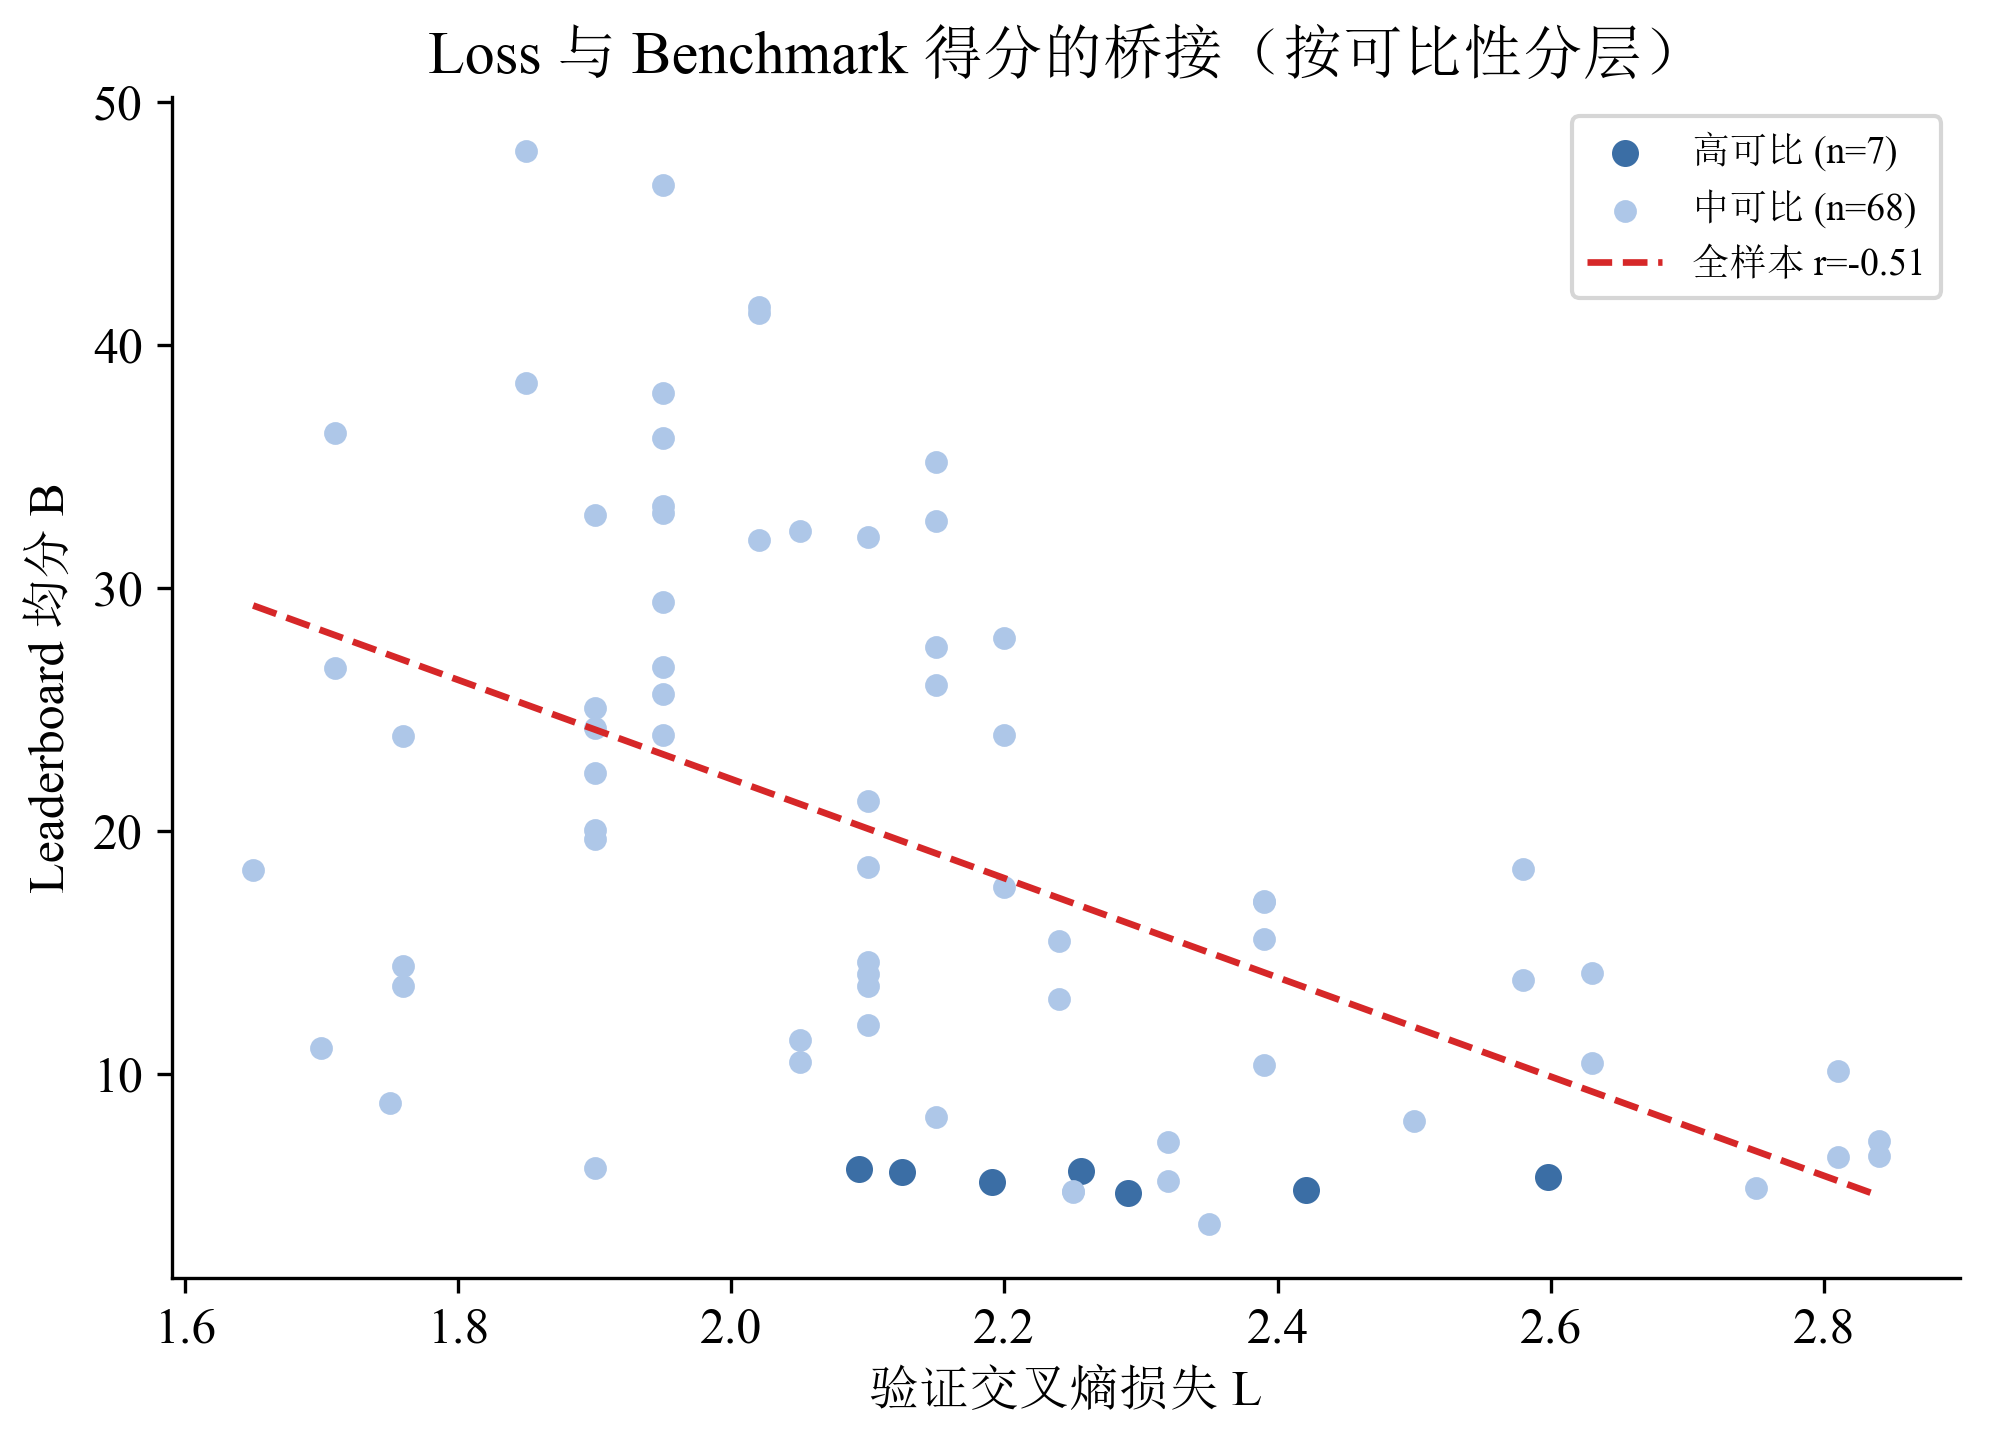
\includegraphics[width=0.60\textwidth]{求解/问题四/图片/图1_Loss_Benchmark映射.png}
  \caption{验证损失与 Leaderboard 均分的映射关系（按可比性分层）}
  \label{fig:p4_map}
\end{figure}

\begin{longtable}{>{\centering\arraybackslash}p{0.16\textwidth}>{\centering\arraybackslash}p{0.10\textwidth}>{\centering\arraybackslash}p{0.13\textwidth}>{\centering\arraybackslash}p{0.13\textwidth}>{\centering\arraybackslash}p{0.13\textwidth}>{\centering\arraybackslash}p{0.10\textwidth}>{\raggedright\arraybackslash}p{0.14\textwidth}}
  \caption{Loss—Benchmark 映射的分层拟合结果（C6，$n=75$）}
  \label{tab:p4_bridge} \\
  \toprule
  可比性 & $n$ & Pearson $r$ & Spearman $\rho$ & 斜率 $b$ & $R^2$ & MAPE(\%) \\
  \midrule
  \endfirsthead
  \caption{Loss—Benchmark 映射的分层拟合结果（续）} \\
  \toprule
  可比性 & $n$ & Pearson $r$ & Spearman $\rho$ & 斜率 $b$ & $R^2$ & MAPE(\%) \\
  \midrule
  \endhead
  \bottomrule
  \endfoot
  高可比 & 7 & $-0.397$ & $-0.607$ & $-0.882$ & 0.16 & 5.6 \\
  中可比 & 68 & $-0.502$ & $-0.509$ & $-19.185$ & 0.25 & 57.3 \\
  全样本 & 75 & $-0.510$ & $-0.549$ & $-20.417$ & 0.26 & 67.8 \\
  C5 对照（全样本） & 43 & $-0.502$ & — & $-16.155$ & — & — \\
\end{longtable}

由表\ref{tab:p4_bridge}可知：（1）损失与能力得分确实负相关（全样本 $r=-0.510$，Spearman $\rho=-0.549$，$p<10^{-6}$），验证了“以损失为目标的资源配置可转化为能力收益”的桥接逻辑；（2）但映射的 $R^2$ 仅 $0.26$、MAPE 高达 $67.8\%$，说明桥接关系是弱关系，其原因是中可比样本的 Loss 来自不同论文的不同验证集、量纲不完全统一；（3）高可比子集（Pythia 同模型同验证集）的斜率最缓（$-0.882$）、MAPE 最低（$5.6\%$），但其得分变化幅度极小（$5.07\sim6.06$），因为这些小规模基础模型在六维基准上都接近随机水平，损失的大幅下降并未转化为得分提升。因此本文的桥接结论仅用于方向性判定与量级估计，不用于把损失数值精确换算为得分。

\textbf{2.规模扩张与非规模技术进步的贡献分解}

面板回归结果见表\ref{tab:p4_panel}，贡献分解如图\ref{fig:p4_decomp}所示。

\begin{longtable}{>{\raggedright\arraybackslash}p{0.28\textwidth}>{\centering\arraybackslash}p{0.10\textwidth}>{\centering\arraybackslash}p{0.14\textwidth}>{\centering\arraybackslash}p{0.12\textwidth}>{\centering\arraybackslash}p{0.10\textwidth}>{\raggedright\arraybackslash}p{0.18\textwidth}}
  \caption{规模系数估计（C1 开源筛选样本，2{,}346 条，2024--2025 年）}
  \label{tab:p4_panel} \\
  \toprule
  子样本 & $n$ & $b_P$（分/10 倍参数） & $b_t$（分/年） & $R^2$ & 说明 \\
  \midrule
  \endfirsthead
  \caption{规模系数估计（续）} \\
  \toprule
  子样本 & $n$ & $b_P$（分/10 倍参数） & $b_t$（分/年） & $R^2$ & 说明 \\
  \midrule
  \endhead
  \bottomrule
  \endfoot
  全样本（年份固定效应） & 2{,}346 & 13.842 & — & 0.475 & 年效应吸收非规模进步 \\
  全样本（线性时间 OLS） & 2{,}346 & 13.842 & 4.844 & 0.475 & 两设定结果一致 \\
  pretrained & 231 & 6.414 & 1.552 & 0.460 & 基础模型 \\
  chat/finetuned & 1{,}497 & 14.853 & 4.680 & 0.484 & 指令/微调模型 \\
\end{longtable}

\begin{figure}[ht]
  \centering
  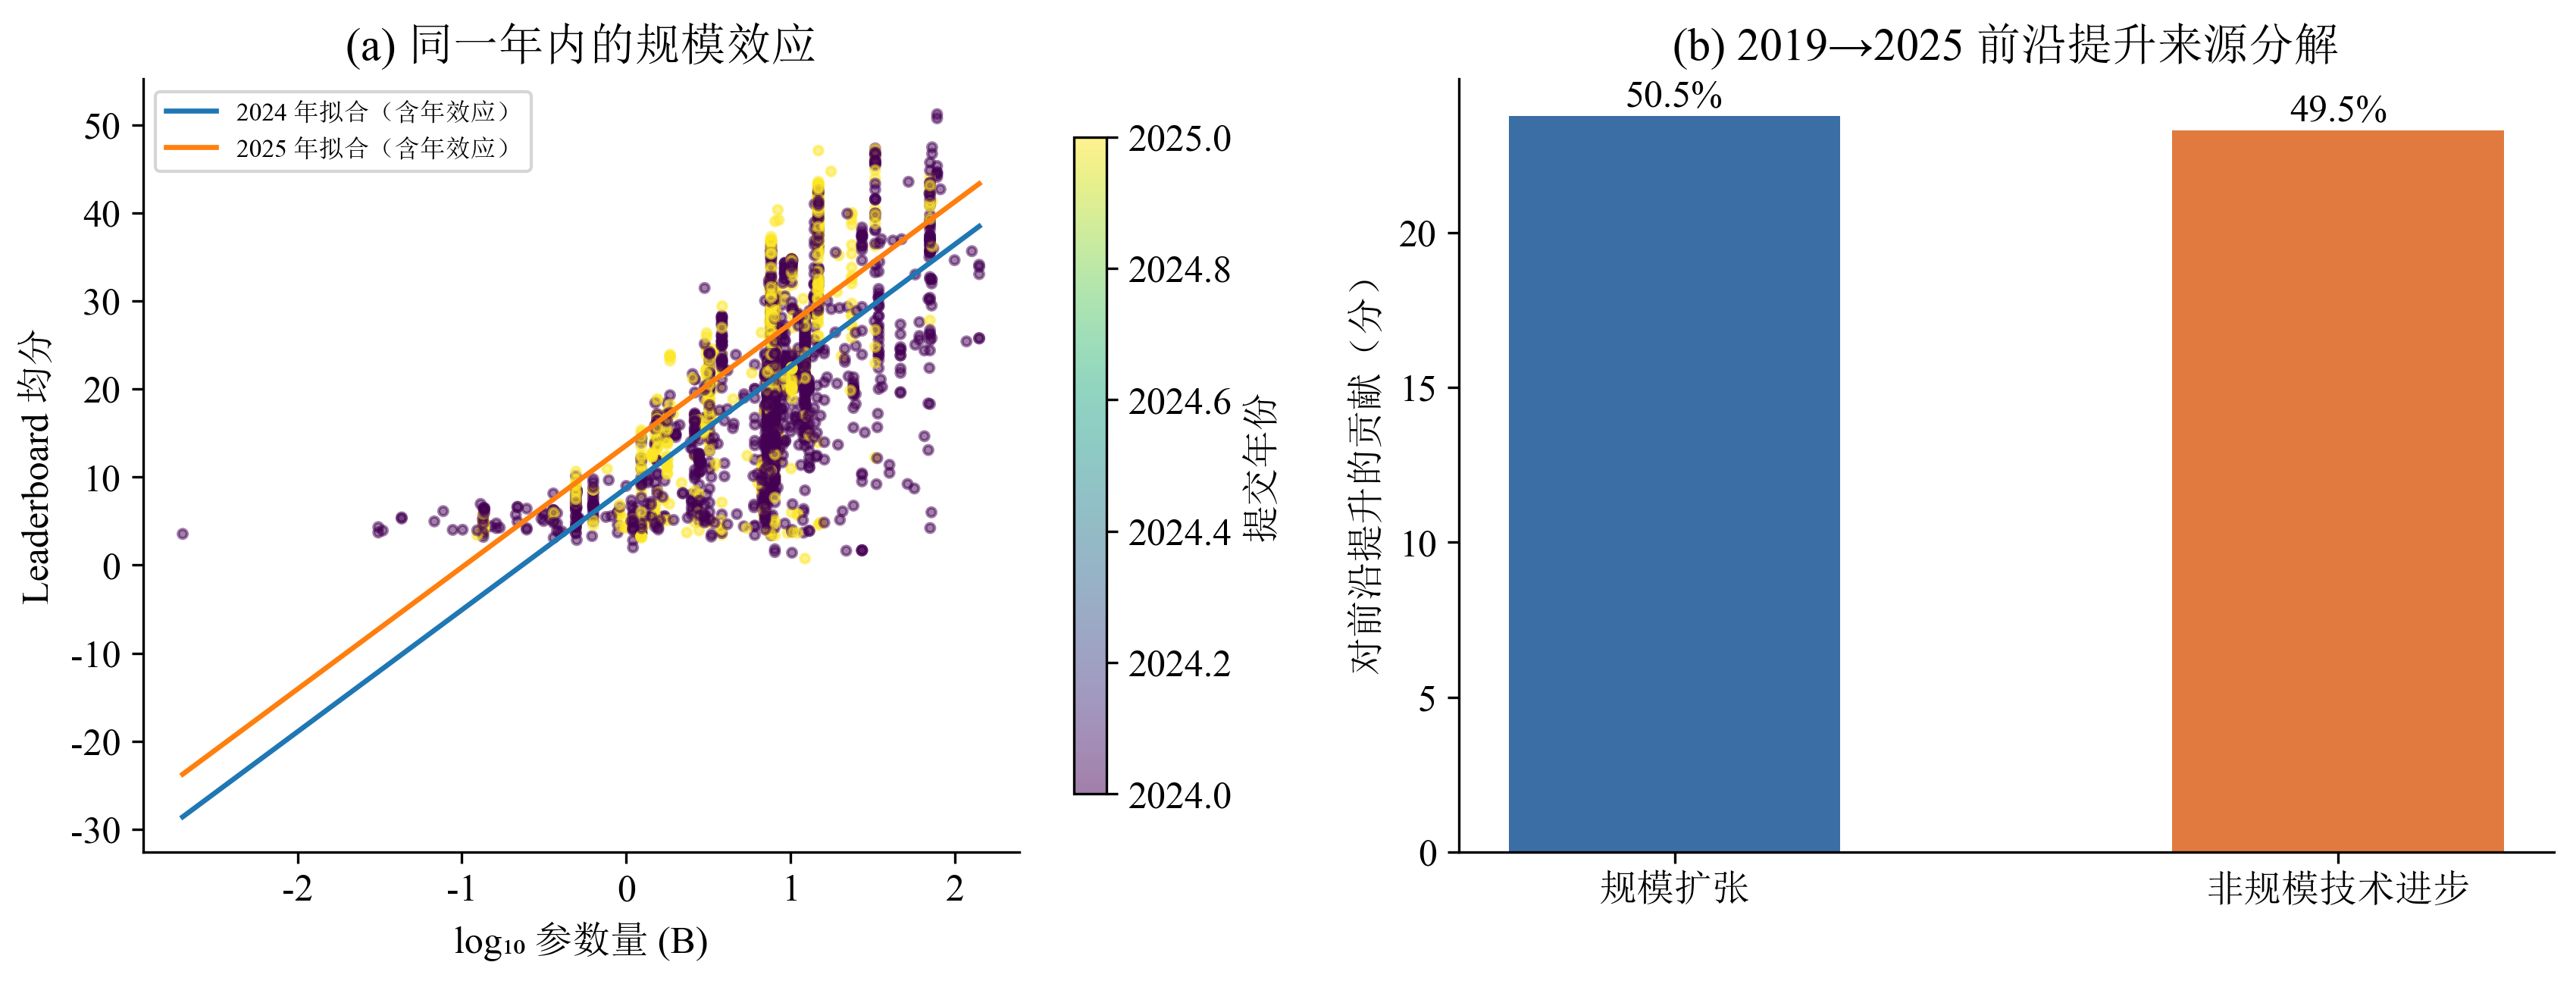
\includegraphics[width=0.92\textwidth]{求解/问题四/图片/图2_规模时间分解.png}
  \caption{规模效应与前沿提升来源分解（左：同一年内的规模效应；右：长周期贡献分解）}
  \label{fig:p4_decomp}
\end{figure}

由表\ref{tab:p4_panel}可知：（1）规模系数 $b_P=13.84$，即参数量每增大 10 倍，六维平均分提升约 $13.8$ 分；非规模技术进步速率 $b_t=4.84$ 分/年。（2）模型类型差异显著：pretrained 子样本的规模系数仅 $6.41$、时间系数 $1.55$，而 chat/finetuned 子样本达 $14.85$ 与 $4.68$，说明经指令微调对齐后的模型对参数规模的利用效率更高，基础模型在同一评测上的得分提升要慢得多。这提示在讨论“规模扩张 vs 技术进步”时必须区分模型类型，否则会因样本构成变化而混淆两者。

在长周期口径（C3，2019--2025）上，以 $b_P=14.10$、$b_t=3.30$（$R^2=0.42$）做 shift-share 分解：前沿由 $5.00$ 升至 $52.08$（提升 $47.08$ 分），其中 $b_P\Delta\log_{10}P=23.77$ 分、残差部分 $23.31$ 分，即\textbf{规模扩张贡献 $50.5\%$、非规模技术进步贡献 $49.5\%$}，二者几乎平分秋色。

但需指出长周期锚点存在口径风险。本文对 C3 做了自洽性审计：比较每行 Average 与其六维均值，发现 13 条记录的差值超过 5（最大差值 $42.3$，为 GPT-3 (175B) 的 Average $=50.0$ 而六维均值仅 $7.67$），说明这些历史条目混入了不同评测标准，已予以剔除。剔除后，在评测标准完全一致的近端窗口（2024-06 至 2024-09，前沿由 $37.99$ 升至 $51.00$）内分解得：前沿模型参数量仅由 $70.6$B 增至 $78.0$B（$\Delta\log_{10}P=0.043$），规模贡献 $0.60$ 分、非规模贡献 $12.41$ 分，即\textbf{该窗口内前沿提升的 $95.4\%$ 来自非规模因素}。这与长周期口径的 $50.5\%$ 形成互补：长期看规模与技术进步各贡献约一半，但在最近一年、模型规模趋于稳定的条件下，能力提升主要由数据工程、对齐方法等非规模因素驱动。

\textbf{3.能力前沿预测}

前沿序列与 logistic 拟合如图\ref{fig:p4_frontier}所示，预测结果与不确定性见表\ref{tab:p4_frontier}。

\begin{figure}[ht]
  \centering
  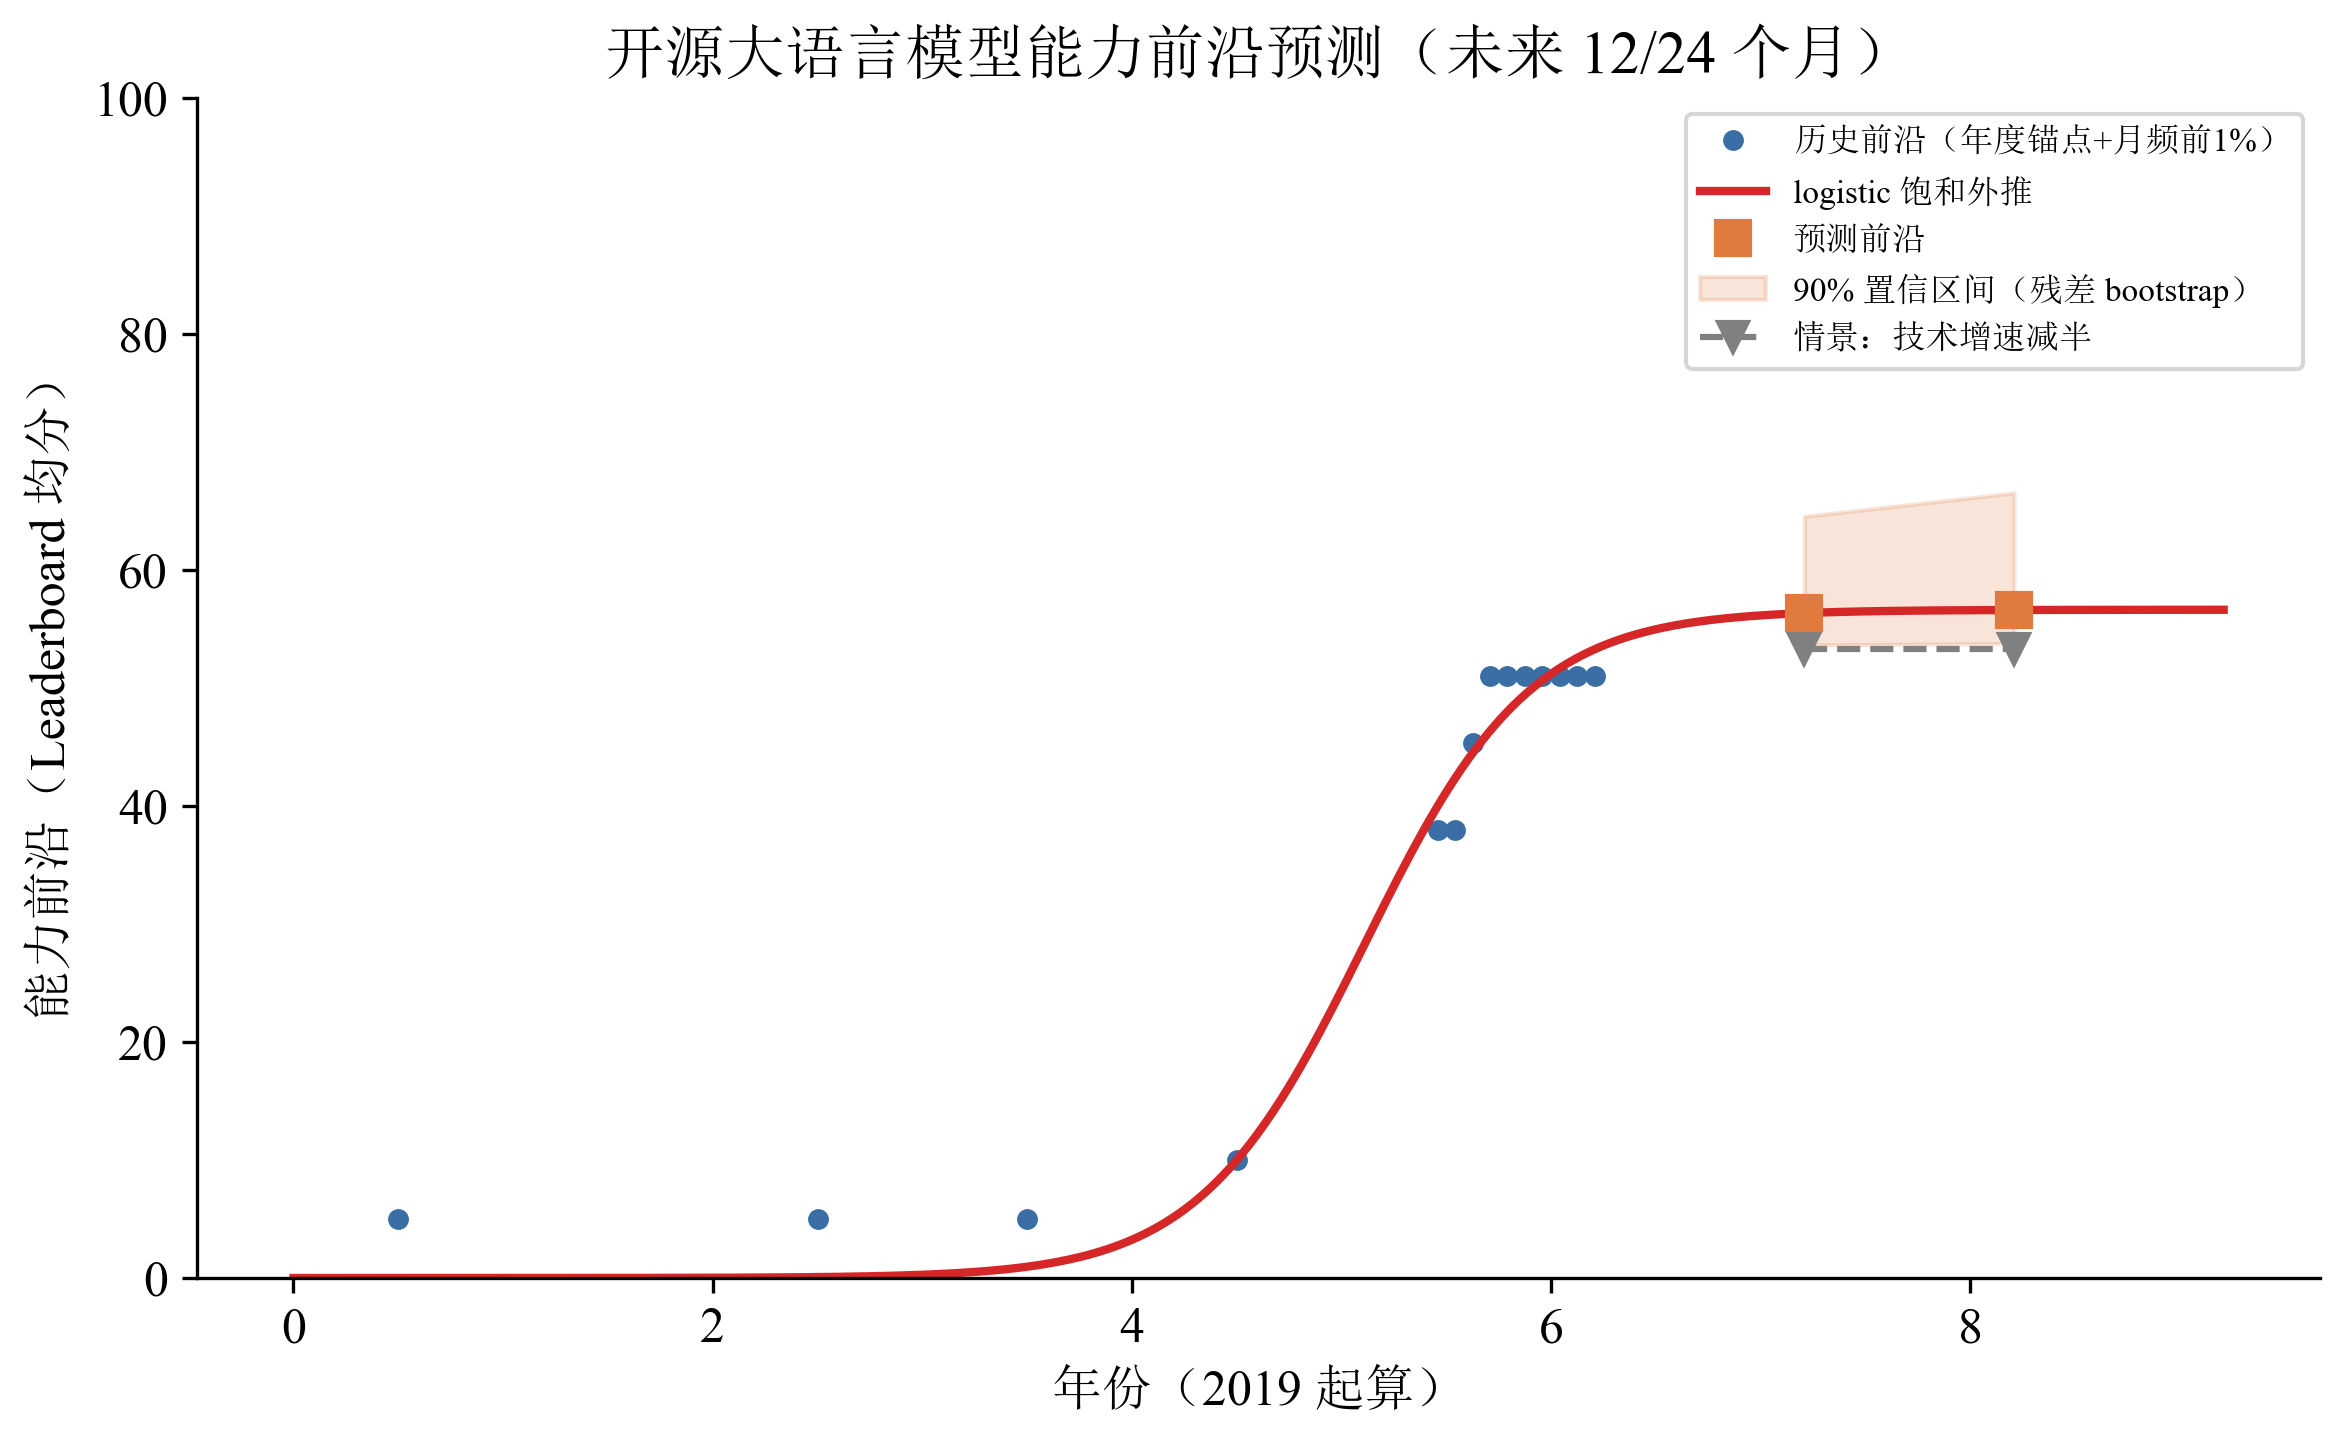
\includegraphics[width=0.72\textwidth]{求解/问题四/图片/图3_能力前沿预测.png}
  \caption{开源大语言模型能力前沿预测（未来 12/24 个月）}
  \label{fig:p4_frontier}
\end{figure}

\begin{longtable}{>{\centering\arraybackslash}p{0.16\textwidth}>{\centering\arraybackslash}p{0.12\textwidth}>{\centering\arraybackslash}p{0.11\textwidth}>{\centering\arraybackslash}p{0.11\textwidth}>{\centering\arraybackslash}p{0.12\textwidth}>{\raggedright\arraybackslash}p{0.22\textwidth}}
  \caption{能力前沿预测及不确定性（满分 100）}
  \label{tab:p4_frontier} \\
  \toprule
  前瞻期 & logistic 预测 & 下界（5\%） & 上界（95\%） & 增速减半 & 结构外推（基准/放缓/扩容） \\
  \midrule
  \endfirsthead
  \caption{能力前沿预测及不确定性（续）} \\
  \toprule
  前瞻期 & logistic 预测 & 下界（5\%） & 上界（95\%） & 增速减半 & 结构外推（基准/放缓/扩容） \\
  \midrule
  \endhead
  \bottomrule
  \endfoot
  $+12$ 个月（2026-03） & 56.33 & 53.62 & 64.52 & 53.27 & 55.84 / 53.42 / 59.99 \\
  $+24$ 个月（2027-03） & 56.59 & 53.75 & 66.52 & 53.27 & 60.69 / 55.84 / 68.99 \\
\end{longtable}

logistic 拟合参数为 $K=56.61$、$r=2.523$、$t_0=5.11$（自 2019 年起算），拟合 $R^2=0.975$。由表\ref{tab:p4_frontier}可知：（1）曲线外推给出未来 12/24 个月前沿约 $56.3$ 与 $56.6$，$90\%$ 置信区间分别为 $[53.6,64.5]$ 与 $[53.8,66.5]$；（2）若算力增长放缓、非规模技术增速减半，前沿将降至 $53.3$ 附近并在两年内基本停滞；（3）结构外推在三种情景下给出 $53.4\sim69.0$ 的区间。两条路线的差异来自“当前前沿是否已接近饱和”这一判断，因此本文以\textbf{区间}而非点值作为结论：未来 12 个月开源模型六维平均分前沿预计达 $53\sim60$，24 个月达 $54\sim69$；若算力增长显著放缓，前沿增速将接近停滞（约 $53\sim56$）。

需强调该预测的局限：本文可用的评测标准一致的窗口仅约 10 个月（2024-06 至 2025-03，Leaderboard v2 已停更），2019--2023 的锚点口径不完全一致（已剔除异常条目），故外推期约为一致窗口的 $1.2\sim2.4$ 倍，结论应理解为情景化区间而非精确点预测。

\textbf{4.逐任务聚合分析}

六维前沿与剩余空间如表\ref{tab:p4_task}与图\ref{fig:p4_task}所示，C8 子任务层面的结果见表\ref{tab:p4_sub}。

\begin{figure}[ht]
  \centering
  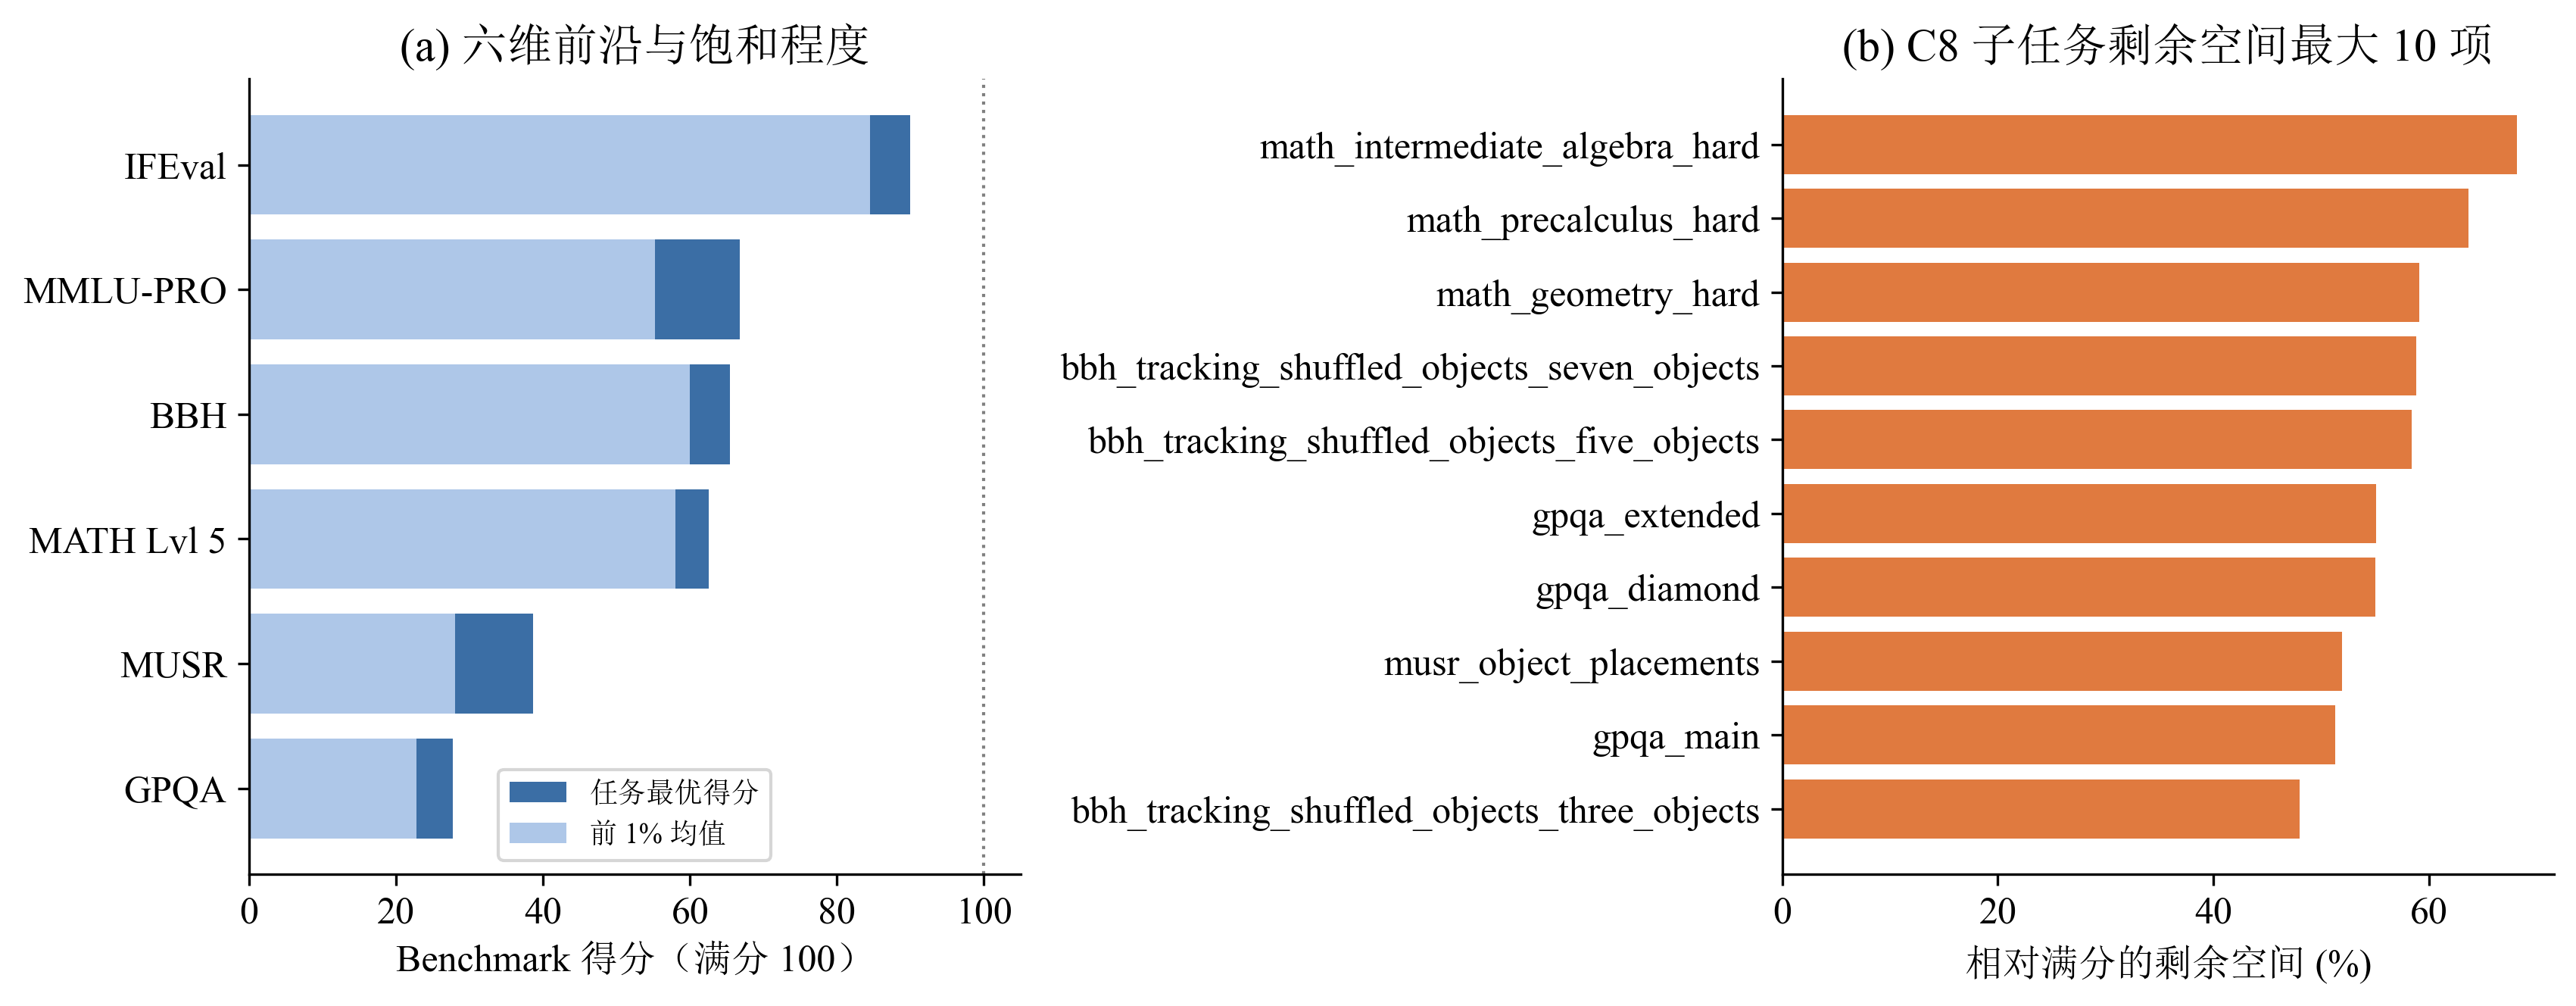
\includegraphics[width=0.92\textwidth]{求解/问题四/图片/图4_逐任务聚合.png}
  \caption{（左）六维 Benchmark 前沿与饱和程度；（右）C8 子任务剩余空间最大的 10 项}
  \label{fig:p4_task}
\end{figure}

\begin{longtable}{>{\centering\arraybackslash}p{0.18\textwidth}>{\centering\arraybackslash}p{0.13\textwidth}>{\centering\arraybackslash}p{0.15\textwidth}>{\centering\arraybackslash}p{0.15\textwidth}>{\raggedright\arraybackslash}p{0.21\textwidth}}
  \caption{六维 Benchmark 逐任务聚合结果（开源筛选集，$n=2{,}346$）}
  \label{tab:p4_task} \\
  \toprule
  任务 & 最优得分 & 前 1\% 均值 & 中位数 & 剩余空间 \\
  \midrule
  \endfirsthead
  \caption{六维 Benchmark 逐任务聚合结果（续）} \\
  \toprule
  任务 & 最优得分 & 前 1\% 均值 & 中位数 & 剩余空间 \\
  \midrule
  \endhead
  \bottomrule
  \endfoot
  IFEval & 89.98 & 84.45 & 43.51 & $10.0\%$ \\
  MMLU-PRO & 66.80 & 55.26 & 25.98 & $33.2\%$ \\
  BBH & 65.47 & 59.95 & 28.52 & $34.5\%$ \\
  MATH Lvl 5 & 62.54 & 58.02 & 9.93 & $37.5\%$ \\
  MUSR & 38.69 & 28.06 & 9.97 & $61.3\%$ \\
  GPQA & 27.74 & 22.80 & 5.70 & $72.3\%$ \\
\end{longtable}

\begin{longtable}{>{\raggedright\arraybackslash}p{0.42\textwidth}>{\centering\arraybackslash}p{0.12\textwidth}>{\centering\arraybackslash}p{0.12\textwidth}>{\centering\arraybackslash}p{0.12\textwidth}>{\raggedright\arraybackslash}p{0.12\textwidth}}
  \caption{C8 子任务层面剩余空间最大的 6 项（原始指标口径）}
  \label{tab:p4_sub} \\
  \toprule
  子任务 & 样本数 & 最优得分 & 前 5\% 均值 & 剩余空间 \\
  \midrule
  \endfirsthead
  \caption{C8 子任务剩余空间最大的 6 项（续）} \\
  \toprule
  子任务 & 样本数 & 最优得分 & 前 5\% 均值 & 剩余空间 \\
  \midrule
  \endhead
  \bottomrule
  \endfoot
  math\_intermediate\_algebra\_hard（MATH） & 962 & 31.79 & 20.11 & $68.2\%$ \\
  math\_precalculus\_hard（MATH） & 962 & 36.30 & 22.89 & $63.7\%$ \\
  math\_geometry\_hard（MATH） & 962 & 40.91 & 28.72 & $59.1\%$ \\
  bbh\_tracking\_shuffled\_objects\_seven（BBH） & 964 & 41.20 & 32.67 & $58.8\%$ \\
  bbh\_tracking\_shuffled\_objects\_five（BBH） & 964 & 41.60 & 31.24 & $58.4\%$ \\
  gpqa\_extended（GPQA） & 961 & 44.87 & 39.74 & $55.1\%$ \\
\end{longtable}

由表\ref{tab:p4_task}与表\ref{tab:p4_sub}可知：（1）六维能力发展极不均衡，指令遵循（IFEval，$89.98$）已接近满分、剩余空间仅 $10.0\%$，而研究生级问答（GPQA，$27.74$）与多轮推理（MUSR，$38.69$）远未饱和，剩余空间分别达 $72.3\%$ 与 $61.3\%$。（2）C8 子任务层面进一步定位了瓶颈：MATH-Hard 中的中级代数、预备微积分、几何三个子任务最优得分仅 $31.8\sim40.9$（该类别 7 个子任务的平均最优得分为 $55.5$，而整体中位数低至 $3.7$），BBH 中“跟踪被洗牌对象”类多步状态推理子任务最优得分约 $41$，GPQA 的 extended 子集为 $44.9$，这些是未来能力增量的主要方向。（3）C8 各类别的中位数普遍远低于最优值（BBH 中位数 $48.8$ 对最优 $81.8$；MATH 中位数 $3.7$ 对最优 $55.5$），说明开源社区的能力分布高度长尾，前列模型与总体水平差距巨大。

\textbf{5.附件 C4 的宏观证据与“算力增长放缓”情景校验}

C4 的宏观趋势如图\ref{fig:p4_c4}所示。

\begin{figure}[ht]
  \centering
  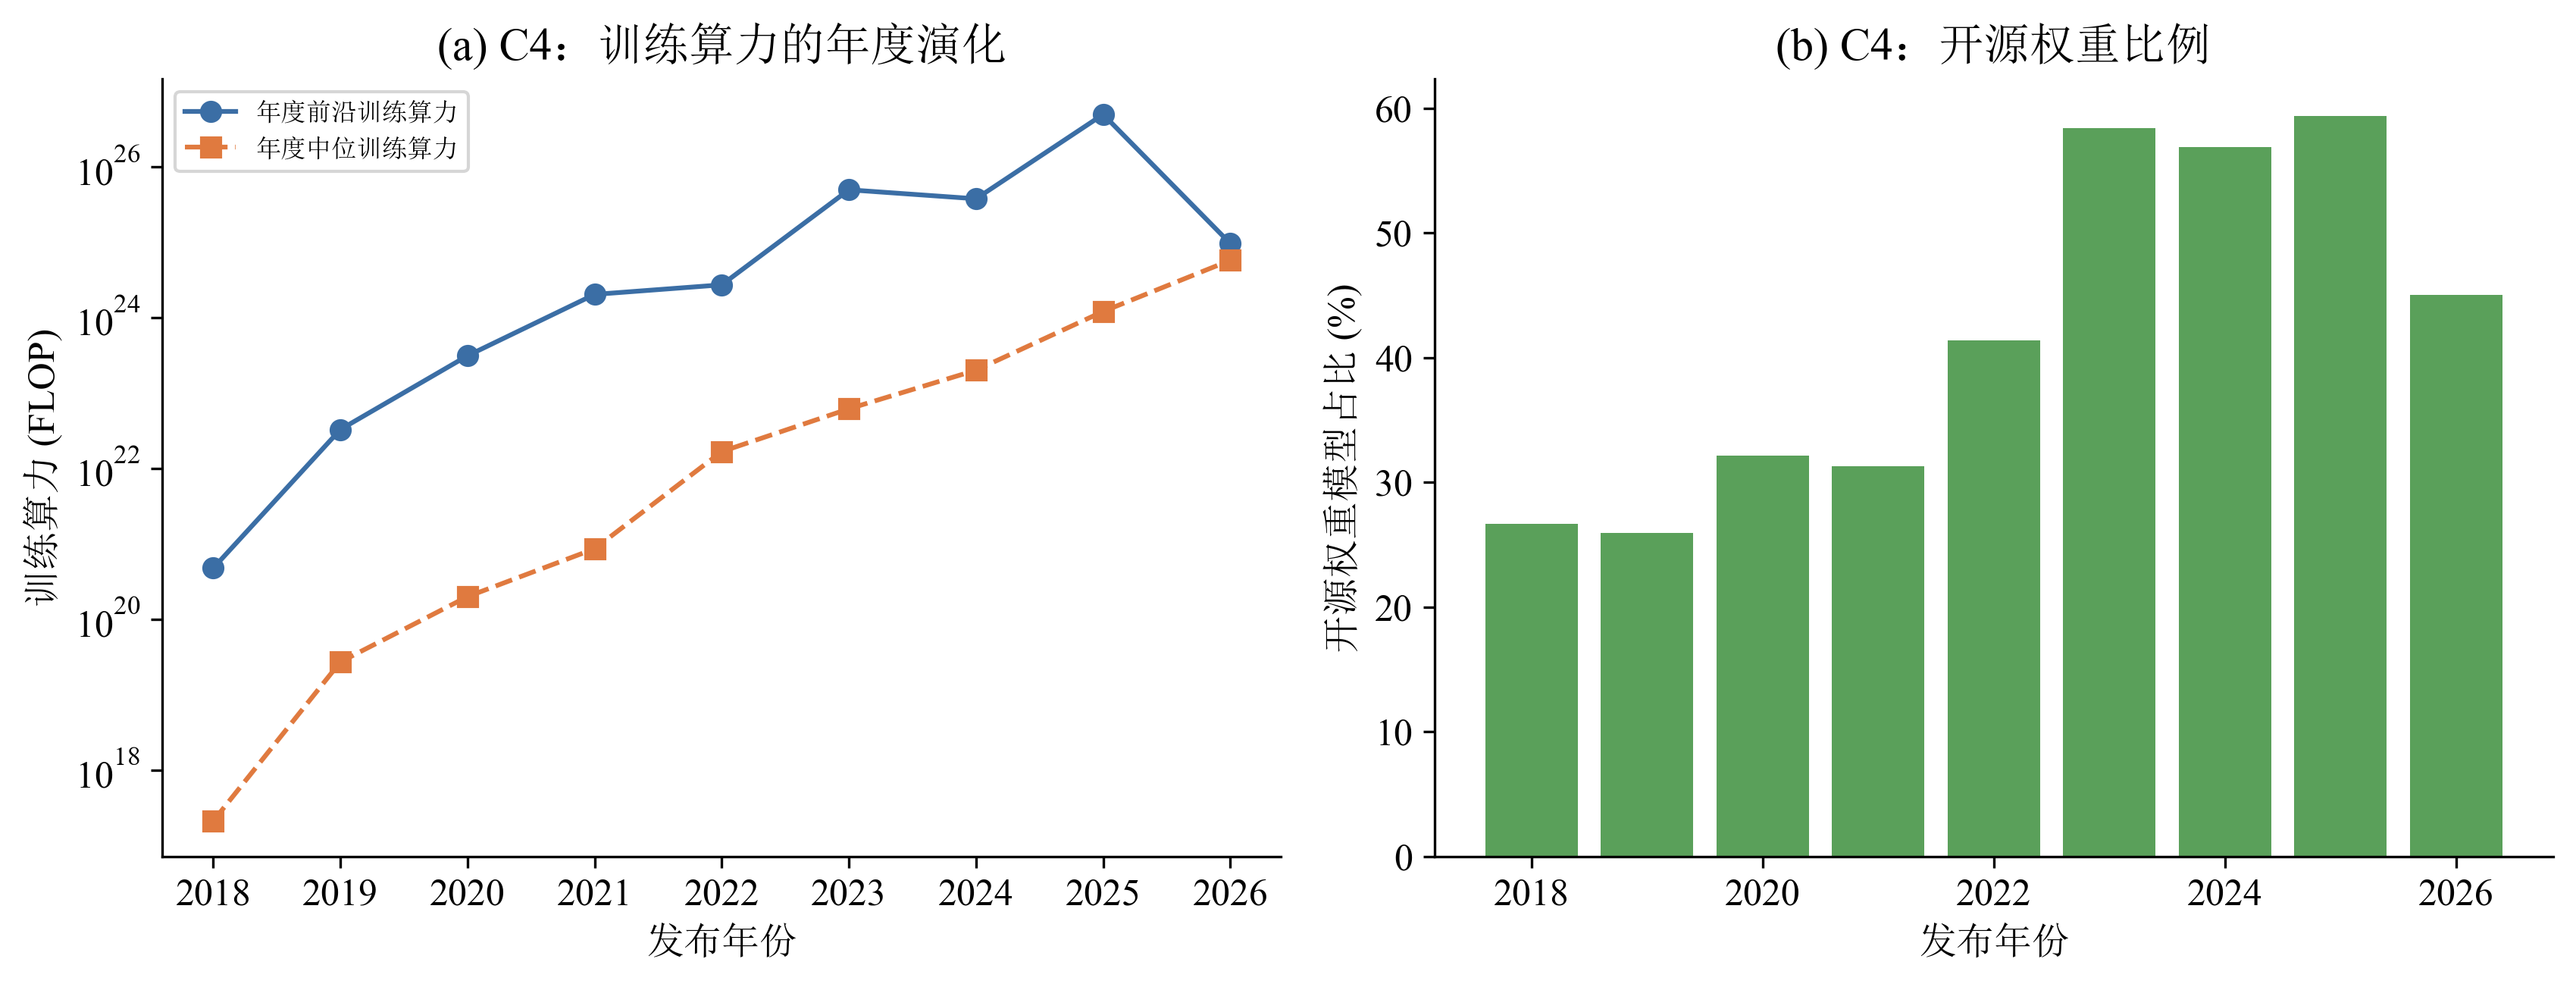
\includegraphics[width=0.92\textwidth]{求解/问题四/图片/图5_C4宏观趋势.png}
  \caption{C4 宏观证据（左：训练算力的年度演化；右：开源权重模型占比）}
  \label{fig:p4_c4}
\end{figure}

由图\ref{fig:p4_c4}可知：（1）C4 中 Language 域模型的前沿训练算力持续增长，对数尺度上的年增速约 $+0.589$ 个数量级（约 $3.88$ 倍/年），表明近年算力投入仍在快速扩张；但年际波动明显（2024 年前沿算力低于 2023 年，2025 年再创新高），说明算力增速并非单调外推、存在阶段性放缓的可能，这也正是本文把“算力增长放缓”作为**情景**（非规模增速减半）而非基准假设、并同时给出基准情景的原因。（2）开源权重模型的占比由 2018 年的 $26.7\%$ 持续上升至 2025 年的 $59.4\%$，说明本文以开源筛选样本刻画“能力前沿”具有良好的代表性与可持续性。（3）C4 中共有 1{,}390 条记录含训练算力、1{,}424 条含训练数据量、2{,}653 条标注开源权重（Yes 1{,}325、No 1{,}328）。需要说明的是，C4 的模型命名体系与 C1 不通用（规范化名称匹配仅命中 1 条），故 C4 仅作宏观尺度证据，不与 C1 逐行合并。

综合以上结果，本节完成了问题四的求解：明确并执行了时间轴、开源筛选与模型类型三类口径；完成了 C8 的逐任务聚合（1{,}860 个模型、37 个子任务维度）并与 C1 交叉校验；建立了分层 Loss—Benchmark 桥接并量化了映射误差；用面板回归分离出规模扩张与非规模技术进步的贡献（长周期各约 $50\%$，近端一致窗口内非规模因素占 $95.4\%$）；给出了未来 12/24 个月能力前沿的情景化预测区间与逐任务瓶颈定位。
